\label{sec:introdutction}
In recent years, the intelligence of a single agent have been significantly improved. To further expand the capabilities of intelligent robots, using multiple robots simultaneously can accelerate many tasks, such as localization, exploration, and mapping.
Decentralized visual simultaneous localization and mapping (DSLAM) can share locations and environmental information between robots, which is an essential task for many multi-robot applications. Cieslewsk et al. \cite{Cieslewski:20187ee} conclude the basic procedure of DSLAM as \cref{fig:all}.

\begin{figure}[h]  
    \centering  
    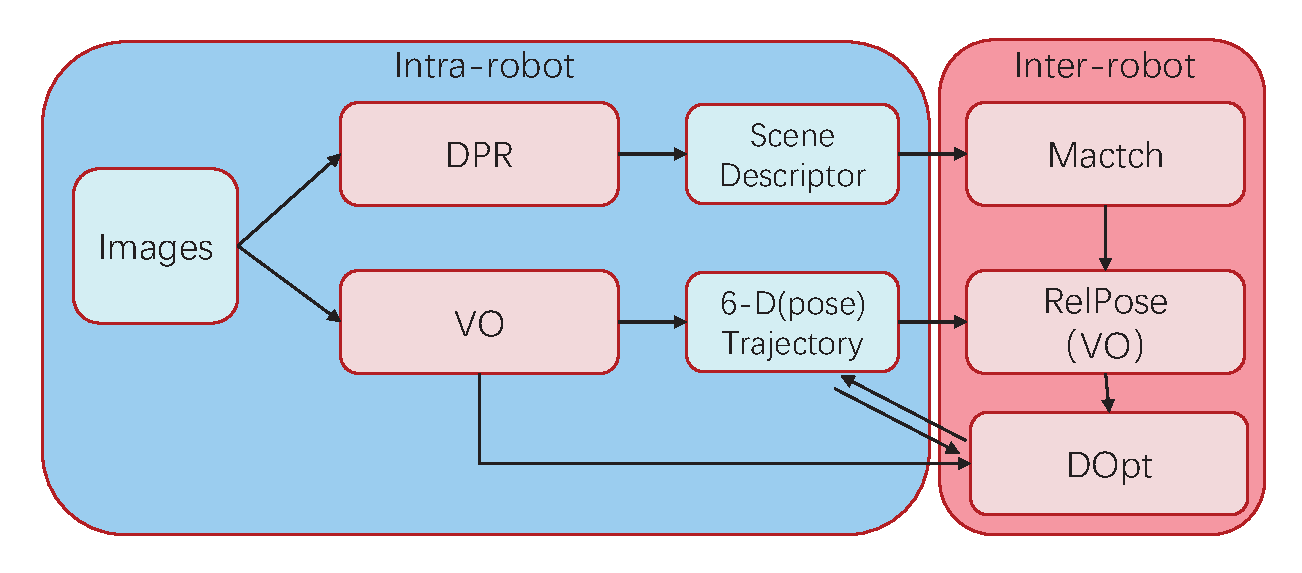
\includegraphics[width=0.85\linewidth]{fig/all.eps}
    \caption{DSLAM framework. \textbf{VO} is used to calculate the intra-robot 6-DoF absolute pose from the input frames. \textbf{DPR} produces a compact image representation to be communicated among robots. \textbf{Match} stage finds out candidate inter-robot place recognition matches.  \textbf{RelPose} requires data from the matched robots and establishes relative poses between the robots trajectories. \textbf{DOpt} does optimization with the trajectories, intra-robot pose measurements from VO and inter-robot relative poses from RelPose, and updates the trajectories.}
    \label{fig:all}
\end{figure}

This framework contains five modules:  Decentralized  Place Recognition (DPR), Visual Odometry (VO), Match, Relative Pose estimation (RelPose) and Decentralized Optimization (DOpt). DPR and VO are intra-robot operations, requiring high computing resources on embedded system. The results of DPR can be used for both intra- and inter-robot loop-closure detection. Match, RelPose and DOpt are inter-robot operations, and consume most of the communication resources of DSLAM sytem. The RelPose part relies on the VO components since it can benefit from re-using VO's data and computing resources.

Cieslewsk et al. \cite{Cieslewski:20187ee} use ORB-SLAM \cite{Mur-Artal:2017281} for VO and NetVLAD \cite{Arandjelovic:2017997} as the DPR component. These two algorithms both consume a large amount of computing and storage resources, and pose a huge challenge to the DSLAM in embedded systems. The DSLAM framework in \cite{Cieslewski:20187ee} is illustrated in \cref{fig:all_pre}.


\begin{figure*}[thb]
    \begin{minipage}[t]{0.5\linewidth}  
    \centering
    \subfigure[DSLAM in \cite{Cieslewski:20187ee}] {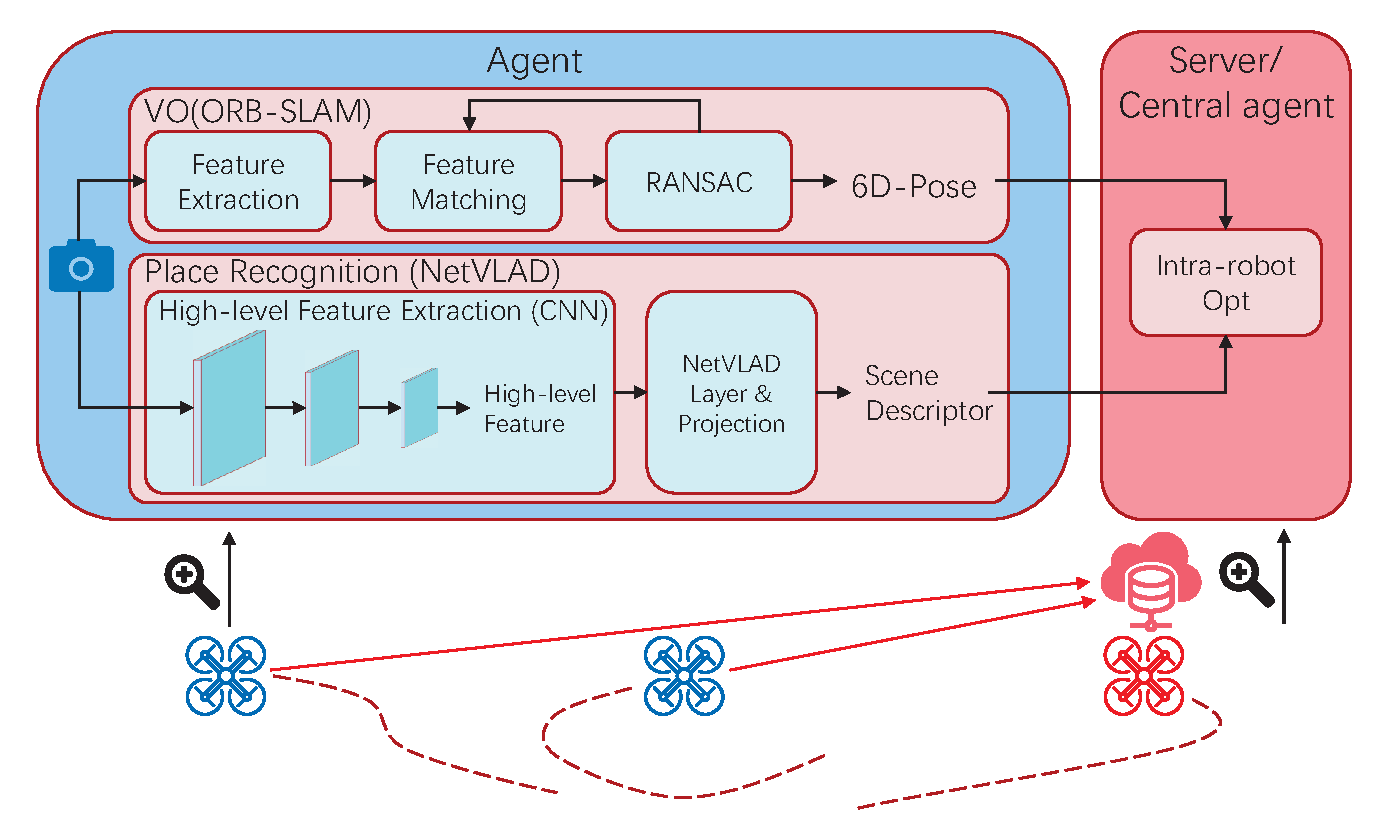
\includegraphics[width=1\textwidth]{fig/overview_pre.eps}\label{fig:all_pre}}
    \end{minipage}
    \begin{minipage}[t]{0.5\linewidth}  
    \centering  
    \subfigure[Our CNN-based DSLAM.] {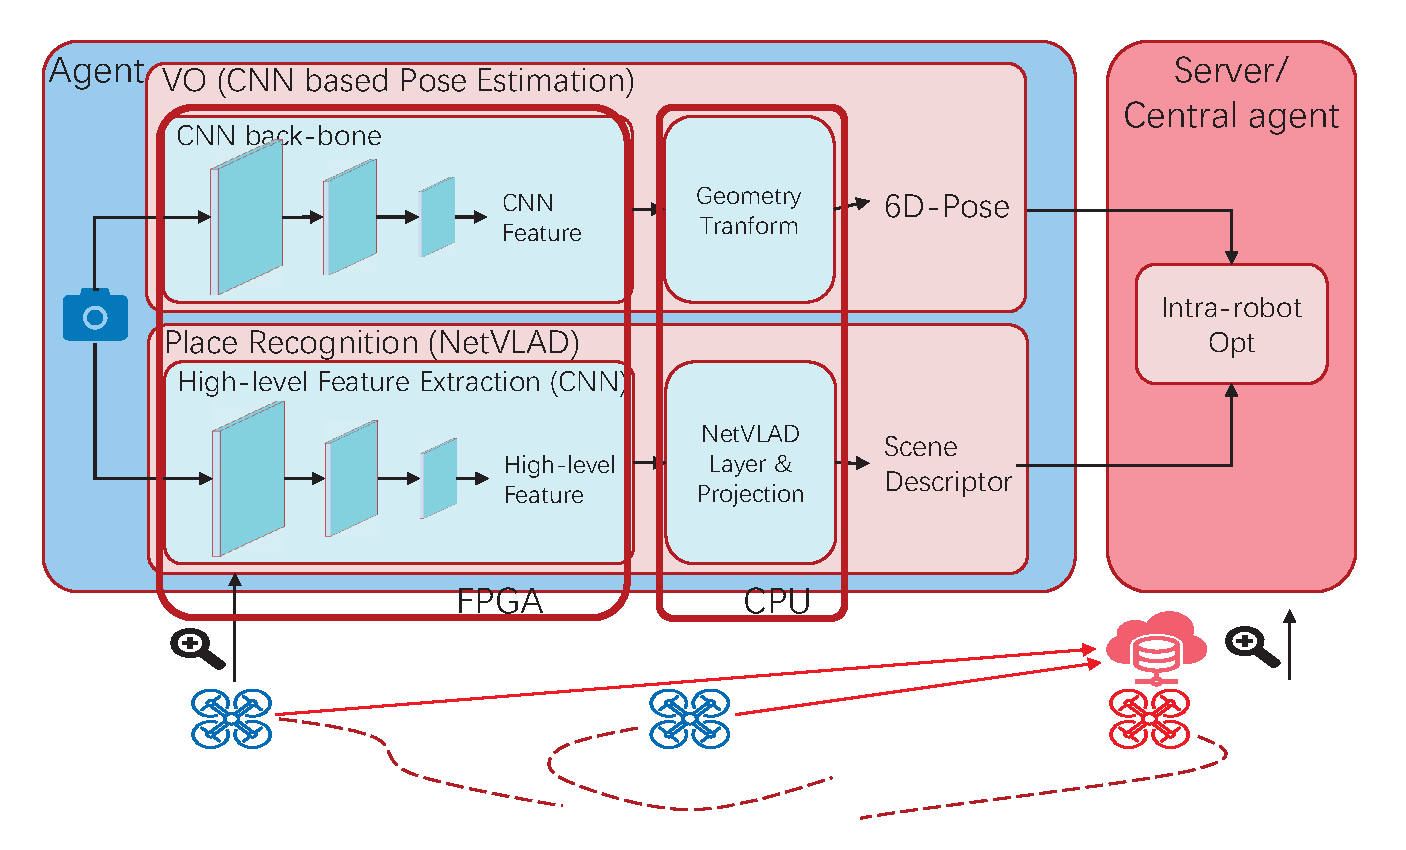
\includegraphics[width=1\linewidth]{fig/overview_us.eps}\label{fig:all_us}} 
    \end{minipage}
    \caption{(a) The previous work uses ORB feature-point-based method to estimate the trajectory from sequences of the stereo camera, and use NetVLAD \cite{Arandjelovic:2017997} to do DPR. (b) Our framework adopt Depth-VO-Feat \cite{Zhan:2018e92} in DSLAM system as the monocular VO, and we use the same method of NetVLAD in \cite{Cieslewski:20187ee} to do DPR. We use the Xilinx Zynq ZU9 MPSoC hardware platform to for deployment.
    }
\label{fig:overview}
\end{figure*}


With the development of CNN, we can reconstruct the depth and pose with the absolute scale from the monocular camera directly, making monocular VO more robust and efficient. And monocular VO methods, like Depth-VO-Feat \cite{Zhan:2018e92}, make DSLAM system much easier to deploy than stereo ones. Besides, some recent advances in deep learning and large-scale labeled vision datasets have significantly improved the accuracy of place recognition (DPR), such as NetVLAD \cite{Arandjelovic:2017997}. However, these previous works only focus on the improvement of network performance, neglecting the deployment of the network on embedded systems.

% Monocular systems are much easier to deploy than binocular systems. The transitional monocular feature point based VO should use complex depth reconstruction methods to compute the absolute scale of the pose scale\cite{pizzoli2014remode}, leading to speed-down. With the development of CNN, we can reconstruct the depth and pose with the absolute scale from the monocular camera directly, making monocular VO more robust and efficient\cite{Zhan:2018e92}. Recent advances in deep learning and the availability of large labelled visual datasets have significantly improved the accuracy of place recognition, such as NetVLAD\cite{Arandjelovic:2017997}. However, previous works concentrate on the accuracy of the CNNs, yet consider little about the deployment CNNs on the embedded system.

Although CNN-based DSLAM systems have many advantages, there are still some key issues to be solved: 1) Embedded systems usually only support fixed-point models. 2) When running multiple CNN models at the same time, the running speed of the system on embedded platforms will decrease, and the slowdown of DPR will lead to the degradation of the final DSLAM accuracy. Therefore, we build up a CNN-based monocular DSLAM system on the embedded FPGA platform with following contributions:
%Though the DSLAM system can benefit from the development of CNN, the fully CNN-based DSLAM system faces some key issues: 1) The embedded system usually support fixed-point CNN. 2) The speed will decline in the embedded system when running several CNN models simultaneously, and the speed-down of DPR will lead to the decline of the final DSLAM accuracy. 

\begin{itemize}
\item To the best of our knowledge, this is the first work to implement all components of monocular DSLAM with CNN. We deploy the system on the Xilinx Zynq ZU9 MPSoC hardware platform with DPU \cite{Tech:2019360}, which is an embedded CNN accelerator. The proposed DSLAM system is illustrated in \cref{fig:all_us}. We also propose a two-stage framework to optimize and deploy a given DSLAM system on the embedded FPGA.
\item As embedded systems impose restrictions on the size of the model, we propose a Pose-Sensitive fixed-point finetune method to divide the VO network into subsets, and adapt different finetune strategies to achieve similar accuracy to the original floating-point VO network. We schedule the fixed-point layers on DPU and the floating-point layers on CPU, so that we can accelerate VO to 10ms/frame.
\item In order to improve the NetVLAD frequency, we propose a cross-component method to schedule the calculation process of VO and DPR, and complete the calculation across the PL and PS of MPSoC to make full use of the embedded platform. And we increase the calculation frequency of NetVLAD from every 12 frames to once every 8 frames.
%\item To increase the NetVLAD frequency, we propose a cross-components scheduling method to scheduling the computation flow across VO and DPR, as well as across the PL and PS of MPSoC to make full use of the embedded platform. We calculate the NetVLAD every 8 input frames from every 12 frames, improving the final accuracy of DSLAM. 
% We also propose a new indicator called loop-closure recall (LCR), which indicates the remaining rate of loop-closure after trajectory merging, to evaluate the performance of trajectory merging. The output result of DSLAM with different NetVLAD frequency is illustrated in \cref{fig:dslamresult}. The tranditional average trajectory error (ATE) can not indicate the performance of trajectory merging in DSLAM.
\end{itemize}

The rest part of this article is organized as follows. \Cref{sec:background} will give the basic idea of CNN-based VO and DPR, as well as the hardware platform. \Cref{sec:hardsoft} will detail the implementation of our two-stage DSLAM framework. The experimental results will be given in \Cref{sec:experiment}. \Cref{sec:conclusion} will conclude this paper.

% The rest part of this article is orgnized as follows. \Cref{sec:background} will give the basic idea of CNN based methods and the hardware architecture of embedded platform, Xilinx Zynq MPSoC. \Cref{sec:hardsoft} will detail the implementation of our pose-sensitive fixed-point fine-tune method and the cross-components scheduling method. The experiment results will be given in \Cref{sec:experiment}. \Cref{sec:conclusion} will conclude this paper.